% Superday Topic B -- principles and results part, version 2.  XeLaTeX:  latexmk -xelatex principles_v2.tex
% Layout spec: talk/superday/OUTLINE.md (binding for v2).  Experiment facts: research/coldstart_C01..C06 PLAN.md and RESULT.md.
\documentclass[t,20pt]{beamer}
\geometry{paperwidth=13.333in,paperheight=7.5in}

% Metropolis inner / outer / colour themes; fonts are set below (Fira Sans + Fira Math from the TeX tree).
\useinnertheme[sectionpage=none,subsectionpage=none]{metropolis}
\useoutertheme[progressbar=none,numbering=none]{metropolis}
\usecolortheme{metropolis}
\usefonttheme{professionalfonts}

\usepackage{fontspec}
\usepackage{unicode-math}
\setsansfont{FiraSans}[Extension=.otf, UprightFont=*-Book, ItalicFont=*-BookItalic,
  BoldFont=*-SemiBold, BoldItalicFont=*-SemiBoldItalic]
\setmainfont{FiraSans}[Extension=.otf, UprightFont=*-Book, ItalicFont=*-BookItalic,
  BoldFont=*-SemiBold, BoldItalicFont=*-SemiBoldItalic]
\setmonofont{FiraMono}[Extension=.otf, UprightFont=*-Regular, BoldFont=*-Medium]
\newfontfamily\mediumfont{FiraSans}[Extension=.otf, UprightFont=*-Medium, ItalicFont=*-MediumItalic]
\setmathfont{FiraMath-Regular.otf}
\newfontfamily\cjkfont{FandolHei-Regular.otf}   % only for one Chinese file name in a source note

\usepackage{tikz}
\usetikzlibrary{arrows.meta,positioning,calc,fit,decorations.markings}
\usepackage{array,booktabs,colortbl}
\usepackage{fancyvrb}

% ------------------------------------------------------------------ colours (OUTLINE.md)
\definecolor{ink}{HTML}{2E2E2E}
\definecolor{sec}{HTML}{6B6B6B}
\definecolor{rulec}{HTML}{C8C8C8}
\definecolor{accent}{HTML}{1F5A96}
\setbeamercolor{normal text}{fg=ink,bg=white}
\setbeamercolor{background canvas}{bg=white}
\setbeamercolor{frametitle}{fg=ink,bg=white}
\setbeamercolor{alerted text}{fg=accent}
\setbeamercolor{structure}{fg=ink}
\arrayrulecolor{rulec}
\setlength{\heavyrulewidth}{0.9pt}
\setlength{\lightrulewidth}{0.9pt}

% ------------------------------------------------------------------ sizes (points are literal: the page is 13.333 x 7.5 in)
\newcommand\titlesize{\fontsize{32}{38}\selectfont}
\newcommand\secsize{\fontsize{16}{20}\selectfont}
\newcommand\nodesize{\fontsize{16}{19}\selectfont\hyphenpenalty=10000\exhyphenpenalty=10000}
\newcommand\notesize{\fontsize{14}{17}\selectfont\hyphenpenalty=10000\exhyphenpenalty=10000}
\newcommand\pnsize{\fontsize{12}{14}\selectfont}

% ------------------------------------------------------------------ grid
\setbeamersize{text margin left=0.85in,text margin right=0.85in}
\setbeamertemplate{navigation symbols}{}
\setbeamertemplate{headline}{}
% Frame title: a fixed-height box, baseline 0.92 in from the top on every page (strut fixes the baseline).
\setbeamertemplate{frametitle}{%
  \nointerlineskip
  \vbox to 1.30in{%
    \vskip 0.50in
    \hbox{{\mediumfont\titlesize\color{ink}\rule{0pt}{0.42in}\insertframetitle}}%
    \vss}%
}
% Page number: bottom right, 12 pt, mid-gray, right edge on the right text margin.
\setbeamertemplate{footline}{%
  \hbox to \paperwidth{\hfill{\pnsize\color{sec}\insertframenumber}\hskip 0.85in}%
  \vskip 0.36in}
\setlength{\parindent}{0pt}
\setlength{\parskip}{0pt}

% ------------------------------------------------------------------ text helpers
\newcommand\key[1]{{\mediumfont\color{accent}#1}}
\newcommand\lead[1]{{\mediumfont #1}}
\newcommand\illus{{\notesize\itshape\color{sec}illustrative}}
\newcommand\file[1]{{\ttfamily\detokenize{#1}}}
\newcommand\sub[1]{\par\vspace{5pt}{\raggedright\secsize\color{sec}#1\par}}
\newenvironment{blist}{%
  \begin{list}{\textcolor{sec}{\textbullet}}{\def\makelabel##1{##1\hfil}%
    \setlength\leftmargin{0.34in}\setlength\labelwidth{0.2in}\setlength\labelsep{0.14in}%
    \setlength\itemsep{16pt}\setlength\parsep{0pt}\setlength\topsep{0pt}\setlength\partopsep{0pt}%
    \setlength\itemindent{0pt}\setlength\listparindent{0pt}\setlength\rightmargin{0pt}}}%
  {\end{list}}
\newcounter{nl}
\newenvironment{nlist}{%
  \begin{list}{\textcolor{sec}{\arabic{nl}}}{\usecounter{nl}\def\makelabel##1{##1\hfil}%
    \setlength\leftmargin{0.40in}\setlength\labelwidth{0.26in}\setlength\labelsep{0.14in}%
    \setlength\itemsep{26pt}\setlength\parsep{0pt}\setlength\topsep{0pt}\setlength\partopsep{0pt}%
    \setlength\itemindent{0pt}\setlength\listparindent{0pt}\setlength\rightmargin{0pt}}}%
  {\end{list}}
\newcolumntype{L}[1]{>{\raggedright\arraybackslash}p{#1}}
\newcommand\thead[1]{\leavevmode{\mediumfont\color{sec}#1}}
\newcommand\gap[1]{\par\vspace{#1}}
% content top: tables and figures start on the frame's top line; a first text line or a [t] minipage is lifted onto it
\newcommand\textfirst{\vspace*{-0.14in}}
\newcommand\colsfirst{\vspace*{-0.37in}}
\newcommand\colsafter{\par\vspace{-0.24in}}
% figures sit on the text block: left edge on the left margin, width exactly the text width
\newcommand\fig[1]{\par\noindent\makebox[\textwidth][l]{\input{#1}}\par}
\AtBeginDocument{\hyphenpenalty=10000\exhyphenpenalty=10000\raggedright}

% ------------------------------------------------------------------ figures: one line width, Stealth tips, square corners
\tikzset{
  x=1in, y=1in,
  >={Stealth[length=7pt,width=5.5pt]},
  every picture/.style={line width=0.9pt},
  grid/.style={trim left=0in, trim right=11.633in-0.9pt},
  box/.style={rectangle, draw=ink, line width=0.9pt, minimum height=0.68in, align=center,
              font=\nodesize, text=ink, inner sep=4pt},
  cb/.style={box},                                  % code part
  lb/.style={box, draw=accent},                     % LLM / Partura part
  pb/.style={box, draw=sec, dashed, text=sec},      % planned, not built
  tint/.style={fill=accent!10},                     % the single 10 % accent tint per figure
  arr/.style={->, line width=0.9pt, draw=ink},
  arrl/.style={->, line width=0.9pt, draw=accent},
  lab/.style={font=\nodesize, text=sec, inner sep=2pt},
  labl/.style={font=\nodesize, text=accent, inner sep=2pt},
  ann/.style={font=\notesize, text=sec, inner sep=1.5pt},        % 14 pt figure annotations
  annl/.style={font=\notesize, text=accent, inner sep=1.5pt},
  anni/.style={font=\notesize, text=ink, inner sep=1.5pt},
  guide/.style={draw=rulec, dotted, line width=0.9pt},            % dotted alignment guides
  mask/.style={fill=white},                                       % label background over a line
  t10/.style={fill=accent!10}, t20/.style={fill=accent!20}, t28/.style={fill=accent!28}, t35/.style={fill=accent!35},
}

\begin{document}

% right-aligned numeric column type (defined outside frames)
\newcolumntype{R}[1]{>{\raggedleft\arraybackslash}p{#1}}

% ================================================================== 1 Title
\begin{frame}[plain]
\begin{tikzpicture}[remember picture,overlay]
  \node[anchor=base west, inner sep=0, align=left, text=ink]
    at ($(current page.north west)+(0.85in,-2.45in)$)
    {\mediumfont\titlesize Partura: an LLM research team\\[2pt]\mediumfont\titlesize that steers a symbolic alpha miner};
  \node[anchor=base west, inner sep=0, text=sec]
    at ($(current page.north west)+(0.85in,-3.45in)$)
    {Principles, design evolution, results C01–C05, C06 running, limitations};
  \draw[rulec] ($(current page.north west)+(0.85in,-3.85in)$) -- ++(11.633in,0);
  \node[anchor=base west, inner sep=0, text=ink]
    at ($(current page.north west)+(0.85in,-4.45in)$) {Xiangyu Wang};
  \node[anchor=base west, inner sep=0, text=sec, font=\secsize]
    at ($(current page.north west)+(0.85in,-4.90in)$) {Trexquant Superday \,·\, Topic B \,·\, 2026-10-30};
  \node[anchor=base east, inner sep=0, text=sec, font=\pnsize]
    at ($(current page.south east)+(-0.85in,0.36in)$) {1};
\end{tikzpicture}
\end{frame}

% ================================================================== 2 Outline
\begin{frame}{Outline}
\textfirst
\begin{nlist}
  \item \lead{Principles} \,—\, pages 3–12
    \sub{Search is cheap, belief is expensive · task · signal card · searcher · current design · verdict rule · integrity}
  \item \lead{Design evolution} \,—\, page 13
    \sub{What changed after each verdict, C01 to C06}
  \item \lead{Results} \,—\, C01–C05 finished \,·\, pages 14–19
    \sub{One table of five verdicts · C05 headline · selection vs.\ out of sample · added heads · why · cost}
  \item \lead{Current experiment} \,—\, \key{C06 running, no results yet} \,·\, pages 20–21
    \sub{Independent auditor · what its result can and cannot show}
  \item \lead{Limitations and conclusion} \,—\, pages 22–23 \,·\, backup 24
\end{nlist}
\end{frame}

% ================================================================== 3 Two speeds
\begin{frame}{Search is cheap, belief is expensive}
\textfirst
LLMs should not write thousands of formulas. They should form beliefs\\
and change \key{where a cheap searcher looks}.
\gap{0.30in}
\fig{figs_v2/loop.tex}
\end{frame}

% ================================================================== 4 Tokens buy beliefs
\begin{frame}{Tokens should buy beliefs, not candidates}
\fig{figs_v2/cost.tex}
\gap{0.30in}
Spend tokens only where an LLM adds value: \key{reading the batches, forming beliefs,}\\
\key{and writing small missions for the searcher}.
\end{frame}

% ================================================================== 5 Task specification
\begin{frame}{Task specification}
\fig{figs_v2/task.tex}
\gap{0.16in}
\lead{Signal}\quad $s_{i,t} = x(\mathcal{D}_{\le t})_i$ \quad {\secsize\color{sec}one number per stock $i$ and day $t$, known after the close of day $t$}
\gap{0.10in}
\lead{Return}\quad $r_{i,t+1} = P_{i,t+2}/P_{i,t+1} - 1$ \quad {\secsize\color{sec}$P$: first-15-minute VWAP; missing if limit-up at the open}
\gap{0.10in}
{\secsize\color{sec}Given: Claude agents (Opus 5.5, Opus 5, Sonnet 5, Haiku 5.5) under a finite token budget; AlphaCube GP;\\
long-only top decile of residuals on five controls, 15 bp per side; \textcolor{accent}{the search sees 2018-01-02 to 2023-08-07 only}.}
\end{frame}

% ================================================================== 6 Signal card
\begin{frame}{A finished output is a signal card}
\begingroup\secsize
\renewcommand\arraystretch{1.45}%
\begin{tabular}{@{}L{2.0in}L{6.0in}L{3.3in}@{}}
\toprule
\thead{Field} & \thead{Content} & \thead{Filled by} \\
\midrule
\lead{Thesis} & mechanism, counterparty, falsifiable prediction, condition under which it fails & \textcolor{accent}{PI (Opus 5.5)}; scored by the auditor (C06) \\
\lead{Implementation} & expression $x$; sign and half-life fixed on train; signal after the close of $t$, trade at the open of $t+1$ & searcher (GP) + reward code \\
\lead{Evidence} & train / valid score; one test read (net excess, $t$); residual read on the five controls; turnover; $|\rho|$ to the known family & deterministic code \\
\lead{Provenance} & mission file, round, seed, code hashes, ledger entry & code (\file{evidence.json}, ledger) \\
\midrule
\multicolumn{3}{@{}l@{}}{\illus\quad the known family as a card: thesis “volatile intraday turnover marks illiquid, speculative names”;} \\[-4pt]
\multicolumn{3}{@{}l@{}}{\phantom{\illus}\quad $x$ = \file{cross_mean(day_std(Amt), 30)}, sign $-1$; evidence and provenance written by code} \\
\bottomrule
\end{tabular}
\endgroup
\gap{0.36in}
Done = all four fields filled \key{and the one test read logged in the ledger}.
\end{frame}

% ================================================================== 7 Searcher as a black box
\begin{frame}{The searcher is a black box with three handles}
\textfirst
Partura never edits AlphaCube. It reaches the search only through \key{three ports}.
\gap{0.22in}
\fig{figs_v2/searcher.tex}
\gap{0.22in}
Same GP in every arm: reward \file{long_neutral} (five controls, 15 bp); depth 2–4.\\
M: budget 192, population 48. Mission runs: population 32, 96 or 128 evaluations.
\end{frame}

% ================================================================== 8 Current design
\begin{frame}{Current design: the main search runs untouched}
\fig{figs_v2/arch.tex}
\end{frame}

% ================================================================== 9 Roles
\begin{frame}{Who reads what, and what each may not do}
\begingroup\secsize
\renewcommand\arraystretch{1.16}%
\begin{tabular}{@{}L{1.90in}L{1.15in}L{3.70in}L{4.38in}@{}}
\toprule
\thead{Role} & \thead{Model} & \thead{Reads} & \thead{Writes; may not} \\
\midrule
\lead{Locate tool} & code & M's batches, train and valid & heads, commonality, ablation \\
\textcolor{accent}{\lead{Anatomist}} & Opus 5 & locate output & alpha subtrees; literature questions \\
\textcolor{accent}{\lead{Librarian}} & Sonnet 5 & the questions & papers before 2023-08-08 only \\
\textcolor{accent}{\lead{PI}} & Opus 5.5 & anatomy, literature, own notes & E, R, N missions; never edits M \\
\textcolor{accent}{\lead{Checker}} & Haiku 5.5 & PI's files & checks, literature dates \\
\textcolor{accent}{\lead{Auditor (C06)}} & Opus 5.5 & mission, heads, known traps & novelty and soundness scores only \\
\bottomrule
\end{tabular}
\endgroup
\gap{0.26in}
Partura reads only its own seed's locate output and earlier missions.\\
Never other seeds, other arms, or test-period numbers.\\
\key{No agent scores its own mission}: scores are code (C05) or a separate auditor (C06).
\end{frame}

% ================================================================== 10 Measuring
\begin{frame}{Measuring the system, not a signal}
\fig{figs_v2/matrix.tex}
\end{frame}

% ================================================================== 11 Verdict rule
\begin{frame}{Verdict rule, fixed before any run}
\textfirst
\lead{Primary}\enspace per seed, the heads of an arm are fused (equal-weight z-rank) into one residual book; its net Sharpe on the test segment, $\mathrm{SR}_X(s)$, is paired with the other arm's on the same seed (8 pairs).
\gap{0.22in}
\begingroup\secsize
\renewcommand\arraystretch{1.30}%
\begin{tabular}{@{}L{3.4in}L{8.05in}@{}}
\toprule
\thead{Verdict} & \thead{Condition (one-sided Wilcoxon signed-rank, $\alpha = 0.05$)} \\
\midrule
\textcolor{accent}{\lead{Partura is better}} & $p(B > A) < 0.05$ and median of $B - A$ above 0 \\
\lead{Partura is worse} & $p(B < A) < 0.05$ and median of $B - A$ below 0 \\
\lead{Cannot tell} & otherwise \\
\bottomrule
\end{tabular}
\endgroup
\gap{0.22in}
\lead{Valid head}\enspace test-segment net excess $> 0$ and $t \ge 2.0$. Heads are de-duplicated greedily on residuals: a candidate with $\rho \ge 0.7$ or $\rho \le -0.5$ to a kept head is dropped.
\gap{0.16in}
{\notesize\color{sec}With 8 pairs the smallest one-sided $p$ is $1/256$. Reported, never in the verdict: forward 2026,\\
B vs.\ B0, valid heads by arm and mission type. PLAN committed 2026-10-28 (ET), before any run;\\
14 dated revisions; RESULT §5 records that none changed a comparison rule.\par}
\end{frame}

% ================================================================== 12 Integrity
\begin{frame}{Integrity: what keeps the experiment honest}
\begingroup\secsize
\renewcommand\arraystretch{1.30}%
\begin{tabular}{@{}L{2.9in}L{8.55in}@{}}
\toprule
\thead{Mechanism} & \thead{How it is enforced} \\
\midrule
\lead{Rules before runs} & PLAN written before any run; later changes only as a dated revision section \\
\lead{Cold start} & agents read only their own seed's files, the PLAN and the code; C06 reuses C05's round-1 files, stated \\
\lead{Information barrier} & Partura sees its own seed's locate output and earlier missions; no other seed, no other arm \\
\lead{Main search untouched} & M never reads Partura; Partura cannot ban or change M \\
\lead{Direction fixed on train} & sign and half-life chosen on train, reused unchanged on valid and test \\
\lead{Ledgered holdout} & test and forward read once per ledger, each read appended; C05: 318 expressions each \\
\lead{Costs} & 15 bp per side; long-only deciles of residuals \\
\lead{Immutable raw results} & evidence never overwritten; infrastructure failure rerun once, unchanged, and logged \\
\bottomrule
\end{tabular}
\endgroup
\gap{0.36in}
\key{No run is repeated because its result looks bad.}
\end{frame}

% ================================================================== 13 Design evolution
\begin{frame}{Design evolution, C01 to C06}
\begingroup\secsize
\renewcommand\arraystretch{1.20}%
\begin{tabular}{@{}L{1.20in}L{5.20in}L{4.70in}@{}}
\toprule
\thead{Step} & \thead{What changed} & \thead{Why this step, from the verdict before} \\
\midrule
\lead{C01} & Partura steers the GP through guidance: priors and neighborhoods on the proposal & first design \\
\lead{C02} & hypotheses tested directly; Partura designs the first population; GP refines locally & C01: belief could not pass through rules matched on writing \\
\lead{C03} & as C02, reward = residual on liquidity, volatility, reversal and known family & C02: style exposure; C01 heads fell 19 to 2 and 13 to 1, C02 7 to 2 and 2 to 0 \\
\lead{C04} & both arms get daily fields; market cap added to the controls; long leg only & C03: both arms find nothing that holds (0 vs.\ 0); search needs inputs it lacks \\
\lead{C05} & \textcolor{accent}{main search runs untouched}; Partura locates, then adds E, R, N missions; it never touches M & C04: a Partura ban removed a family the plain GP kept (53 vs.\ 173 discoveries) \\
\lead{C06} & + independent auditor scores each mission before it runs; M and A reused from C05 & C05: better in selection, not out of sample; screen before a run \\
\bottomrule
\end{tabular}
\endgroup
\gap{0.20in}
{\notesize\color{sec}Sources: each PLAN §1 (C02–C06) and each RESULT §1 or §4 (C01–C05).\par}
\end{frame}

% ================================================================== 14 Results table
\begin{frame}{Five comparisons, one table}
\begingroup\secsize
\renewcommand\arraystretch{1.30}%
\begin{tabular}{@{}L{1.25in}L{4.85in}L{2.45in}L{2.55in}@{}}
\toprule
\thead{Experiment} & \thead{Design, one line} & \thead{Primary verdict} & \thead{Test-period key number} \\
\midrule
\lead{C01} & AlphaCube alone vs.\ with Partura's guidance files; 3 rounds, 8 seeds & \textcolor{accent}{Partura is worse} & valid heads: A 19, B 13 \\
\lead{C02} & Partura v2: hypotheses tested directly, designed first population, GP refinement; 8 seeds & \textcolor{accent}{Partura is worse} & new valid heads: A 7, B 2 \\
\lead{C03} & as C02, reward = residual on liquidity, volatility, reversal, known family; 16 seeds & Cannot tell & valid heads: A 0, B 0 \\
\lead{C04} & both arms get daily fields; market cap added to the controls; long leg only; 16 seeds & Cannot tell & median B − A −0.17\newline p(B worse) 0.11 \\
\lead{C05} & main search untouched; Partura adds E, R, N missions; 8 seeds & Cannot tell & median B − A +0.08\newline p(B better) 0.42 \\
\bottomrule
\end{tabular}
\endgroup
\gap{0.22in}
{\notesize\color{sec}Sources: research/coldstart\_C0x/RESULT.md §1 and §2. C01 and C02 count valid heads (test-period net excess $> 0$, $t \ge 2$); C02 counts only heads not correlated with C01's.\\
C04 and C05 use the per-seed fused-book test Sharpe as primary, 16 and 8 seed pairs.\par}
\end{frame}

% ================================================================== 15 C05 headline
\begin{frame}{C05 headline: cannot tell}
\textfirst
\lead{Primary verdict on the test segment:} \key{cannot tell}, as pre-registered.
\gap{0.20in}
\begingroup\secsize
\renewcommand\arraystretch{1.40}%
\begin{tabular}{@{}L{4.00in}L{3.30in}L{3.80in}@{}}
\toprule
\thead{Measure, B against A} & \thead{Test 2023-08-08 to 2025-12-31 (verdict)} & \thead{Forward 2026, 0.67 years (report only)} \\
\midrule
Median difference, B $-$ A & +0.08 & −0.39 \\
One-sided $p$ (B worse) & 0.63 & 0.039 \\
Seeds where B is higher & 5 of 8 & 2 of 8 \\
Mean fused-book Sharpe, A & 0.44 & 0.87 \\
Mean fused-book Sharpe, B & 0.44 & 0.29 \\
\bottomrule
\end{tabular}
\endgroup
\gap{0.26in}
One-sided $p$ (B better) on test is 0.42. Forward figures are reported as the PLAN requires and do not change the verdict.\\
\key{Both arms are level on test.} The forward 2026 gap is reported, but it covers only 0.67 years.
\end{frame}

% ================================================================== 16 Selection vs out of sample
\begin{frame}{Better in selection, not out of sample}
\fig{figs_v2/selection.tex}
\end{frame}

% ================================================================== 17 Added heads
\begin{frame}{Added heads were weaker out of sample}
\begingroup\secsize
\renewcommand\arraystretch{1.25}%
\begin{tabular}{@{}L{5.30in}L{1.85in}L{1.95in}L{2.00in}@{}}
\toprule
\thead{Heads added by the arm} & \thead{A: plain GP} & \thead{B0: mechanical} & \thead{B: Partura} \\
\midrule
Heads added, including R replacements & 101 & 56 & 94 \\
Pass the test rule (net excess $> 0$, $t \ge 2.0$) & 15 of 101 & 10 of 56 & \textcolor{accent}{3 of 94} \\
Mean single-head test Sharpe & 0.80 & 0.69 & \textcolor{accent}{0.32} \\
Mean single-head forward Sharpe (report only) & 0.70 & 0.36 & 0.01 \\
In-sample score of the added heads (group level) & 1.04 & 1.07 & 1.01 \\
Test Sharpe, E missions (fixed core, new periphery) & — & 0.65 & \textcolor{accent}{0.31} \\
Test Sharpe, N missions (B0: plain GP) & — & 0.54 & 0.19 \\
\bottomrule
\end{tabular}
\endgroup
\gap{0.26in}
{\notesize\color{sec}Same-seed heads are correlated: these rows describe the arms, they are not tests. Source: C05 RESULT §1, §3, §4b.\par}
\end{frame}

% ================================================================== 18 Why
\begin{frame}{Why? Hypotheses, not tests}
\textfirst
\key{Formed after reading the test period (C05 RESULT §4b). Not tested.}
\gap{0.14in}
\begin{nlist}
  \item \lead{Goodhart.} Partura optimizes a leaky in-sample reward better than blind search: convex transforms rebuild volatility, and at least 5 of 25 E cores are size or volatility rewrites.
    \sub{For example \file{LogFloatShares}, \file{inv(LogFloatShares)}, \file{day_var(Ret)}. C06 leaves the reward unchanged.}
  \item \lead{Researcher degrees of freedom.} Same locate output: 0.65 under the mechanical rule (B0), 0.31 when the LLM picks cores, seeds and periphery (B).
    \sub{Choices made on train and valid, not counted as trials, yet many tests on the same data.}
  \item \lead{Crowded priors, weaker.} Papers before 2023-08-08 may describe effects already traded.
    \sub{N heads that are, or contain, a full seed score about 0.05 on test; a small sample.}
\end{nlist}
\end{frame}

% ================================================================== 19 Cost
\begin{frame}{What C05 cost, measured}
\begingroup\secsize
\renewcommand\arraystretch{1.40}%
\begin{tabular}{@{}L{5.90in}L{5.23in}@{}}
\toprule
\thead{Item, 8 seeds} & \thead{Measured value} \\
\midrule
Extra paid evaluations: A / B0 / B & 4,371 / 4,579 / \textcolor{accent}{4,891} \\
GP run time, excluding locate and R: M / A / B0 / B & 6.2 h / 8.2 h / 6.3 h / \textcolor{accent}{6.8 h} \\
LLM agent calls, arm B (including reruns) & \textcolor{accent}{101} \\
LLM output tokens, arm B & \textcolor{accent}{13.21 M} \\
Cache read / cache write, arm B & 630 M / 47.8 M \\
\bottomrule
\end{tabular}
\endgroup
\gap{0.30in}
M, A and B0 used no LLM tokens; every LLM figure above is arm B's.\\
{\notesize\color{sec}Source: C05 RESULT §2, which gives token totals in 10k and 100M units; converted here, cache write rounded.\par}
\end{frame}

% ================================================================== 20 C06 design
\begin{frame}{C06: an independent auditor screens missions}
\fig{figs_v2/cflow.tex}
\end{frame}

% ================================================================== 21 C06 status
\begin{frame}{C06 is running; no results yet}
\textfirst
\key{Status: running. No C06 result appears in this deck.}
\gap{0.18in}
\begin{blist}
  \item \lead{Design.} Arm C (Partura with auditor) against A (plain GP), 8 seeds, same verdict rule as C05. M and A are reused from C05, not rerun.
  \item \lead{Three fixes against C05.} The E reward no longer counts the core's family; an R variant can enter as a new head; R replacements run to the end of their chain.
\end{blist}
\gap{0.30in}
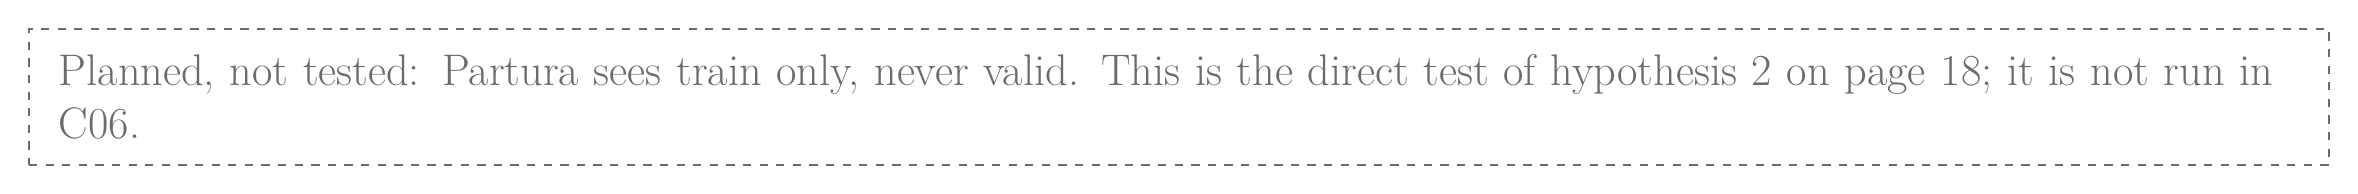
\begin{tikzpicture}[x=1in, y=1in]
  \node[pb, minimum width=11.50in, text width=11.20in, anchor=north west, align=left, inner sep=8pt] at (0,0)
    {{\mediumfont Planned, not tested:} Partura sees train only, never valid. This is the direct test of hypothesis 2 on page 18; it is not run in C06.};
\end{tikzpicture}
\gap{0.36in}
\begingroup\secsize
\key{Caveat.}\enspace The test period has been read five times.\\
C06 was designed after reading C05's test result, so a win on test would be discounted.\\
The clean check is data after 2026-09-16, which is not used here.
\endgroup
\end{frame}

% ================================================================== 22 Limitations
\begin{frame}{Known limitations}
\textfirst
\begin{blist}
  \item \lead{Test segment read five times.} C01–C05 each read it; C06 was designed after reading C05's test result.
  \item \lead{Low power.} Eight seed pairs; the smallest one-sided $p$ is $1/256$. Forward 2026 is only 0.67 years.
  \item \lead{Fixed information schedule.} Round $k$ sees M's first $k$ batches: not true asynchrony. Literature dates are spot-checked only.
  \item \lead{Reward unchanged.} C06 blocks exploits with an LLM auditor, which may over- or under-reject. C05's E reward counted the family in the controls, unlike its library rule (fixed in C06).
  \item \lead{Survivorship; A-shares, long-only.} The store has no delisted names; T+1 and limit-up names cannot be bought. Both arms share this.
\end{blist}
\end{frame}

% ================================================================== 23 Conclusion
\begin{frame}{What the evidence supports so far}
\textfirst
\begin{nlist}
  \item \lead{No win on the primary metric.} Partura never beat plain GP on its pre-registered metric: two \key{worse} (C01, C02), three \key{cannot tell} (C03–C05).
  \item \lead{The floor held in C05.} With the main search untouched, the fused test book was not worse than A: 0.44 for both.
  \item \lead{One construction survived.} C04's feature, daily return scaled by limit width, came from Partura and survived GP refinement:
    12 of its 14 descendants had positive net excess on test. GP refinement reversed the sign Partura wrote, and the family's forward mean was 0.04.
  \item \lead{Still open.} Whether an independent auditor (C06) closes the gap between selection and test. The clean test is data after 2026-09-16.
\end{nlist}
\end{frame}

% ================================================================== 24 Backup
\begin{frame}{Backup: C05 per-seed numbers}
\begingroup\notesize
\renewcommand\arraystretch{1.25}%
\begin{tabular}{@{}L{2.35in}*{8}{R{0.93in}}@{}}
\toprule
\thead{Fused-book Sharpe} & \thead{801} & \thead{802} & \thead{803} & \thead{804} & \thead{805} & \thead{806} & \thead{807} & \thead{808} \\
\midrule
M, test & +0.44 & +0.50 & +0.31 & −0.64 & +0.20 & +1.78 & −0.13 & −0.07 \\
A, test & +0.41 & +0.34 & +0.72 & −0.06 & +0.64 & +0.93 & +0.05 & +0.51 \\
B0, test & +0.48 & +0.46 & +0.87 & −0.57 & +0.34 & +1.43 & +0.16 & +0.03 \\
B, test & +0.52 & +0.74 & +0.61 & −0.75 & +0.94 & +1.15 & +0.10 & +0.19 \\
\textcolor{accent}{B $-$ A, test} & \textcolor{accent}{+0.11} & \textcolor{accent}{+0.40} & \textcolor{accent}{−0.11} & \textcolor{accent}{−0.69} & \textcolor{accent}{+0.31} & \textcolor{accent}{+0.22} & \textcolor{accent}{+0.05} & \textcolor{accent}{−0.32} \\
\midrule
A, forward 2026 & +0.58 & +1.02 & +0.81 & +0.43 & +0.36 & +1.02 & +0.78 & +1.94 \\
B, forward 2026 & +0.93 & +0.76 & +0.24 & −1.19 & −0.06 & +1.36 & +0.41 & −0.16 \\
B $-$ A, forward 2026 & +0.35 & −0.26 & −0.57 & −1.62 & −0.42 & +0.34 & −0.36 & −2.10 \\
\bottomrule
\end{tabular}
\endgroup
\gap{0.22in}
{\notesize\color{sec}No head counts as 0 (RESULT §2 convention). Test: 2023-08-08 to 2025-12-31. Forward: 2026, report only.
Source: research/coldstart\_C05/RESULT.md §2, per-seed table.\par}
\end{frame}

\end{document}
